\documentclass[
	hyperref={
		pageanchor=false,
		bookmarks=false,
		pdfpagelabels=false},
	aspectratio=169,
	]{beamer}
\usepackage{pgfpages}									% for producing notes
% \setbeameroption{show notes on second screen}
% \usetheme[progressbar=frametitle]{metropolis}           % Use metropolis theme
\useinnertheme{metropolis}
\useoutertheme[progressbar=frametitle]{metropolis}
\usecolortheme{metropolis}
\definecolor{lightblue}{RGB}{0,190,255}					% Define colors of corporate design of University of Stuttgart
\definecolor{midblue}{RGB}{0,81,158}
\definecolor{anthrazit}{RGB}{62,68,76}
\setbeamercolor{alerted text}{fg=midblue}				% Set colors
%\setbeamercolor{normal text}{fg=anthrazit}
\usepackage{caption}									% Use \captionof
\usepackage{tikz}
\usetikzlibrary{shapes,arrows.meta}
\usetikzlibrary{calc}
\usepackage{amsmath}									% Use of align which is assumer superior to eqnarray
\usepackage{tabularx}									% Needed for using align in tabular-environment
\usepackage{array}										% Center text in column with specified width
\newcolumntype{P}[1]{>{\centering\arraybackslash}p{#1}}
% \usepackage{colortbl}									% Specify \arrayrulecolor for use in timeline
 \usepackage{booktabs}									% Use of \toprule
 \usepackage{tabu}
\title{Crashing simulated planes is cheap: Can simulation detect robotics bugs early?}
\date{May 10, 2018}
\author{Sangwon Hyeon, Caroline, Andreas Poppele}
% \institute{KIXLAB, Korea Advanced Institue of Science and Technology}
%\logo{\includegraphics{images/unistuttgart_logo_de.jpg}}

\usepackage[T1]{fontenc} % utf8 <- produce real utf8 characters
\usepackage[utf8]{inputenc} % utf8 <- accept utf8 input characters
\usepackage[english]{babel}
\usepackage{anyfontsize} % mute warnings?
\usepackage{silence} % Error / Warning filter
\usepackage{textcomp} % Fix font warning
\usepackage[numbers]{natbib} % use natbib for \citeauthor{} and Co.

\makeatletter % Enable footnotes without marker
\def\blfootnote{\gdef\@thefnmark{}\@footnotetext}
\makeatother
%---------------------------------
% Silence Warning
%---------------------------------
\WarningFilter{biblatex}{Patching footnotes failed}
\WarningFilter{beamerthememetropolis}{You need to compile with XeLaTeX or LuaLaTeX to use the Fira fonts}

\NoHyper % remove warnings - but no links


\begin{document}
	\maketitle

	\begin{frame}
		\frametitle{Outline}
		\tableofcontents
	\end{frame}
\setlength{\belowcaptionskip}{-1.5em}

%---------------------------------
% Section Introduction
%---------------------------------
\section{Introduction}
	\begin{frame}{Introduction}
		Intro
	\end{frame}

%---------------------------------
% Section Background
%---------------------------------
\section{Background}
	\begin{frame}{Background}
		Background
	\end{frame}

%---------------------------------
% Section Related Work
%---------------------------------
\section{Related Work}
	\begin{frame}{Related Work}
		Related
	\end{frame}

%---------------------------------
% Section Methodology
%---------------------------------
\section{Methodology}
	\begin{frame}{Methodology}
		Methods
	\end{frame}

%---------------------------------
% Section Results
%---------------------------------
\section{Results}
	\begin{frame}{Results}
		Results
	\end{frame}

%---------------------------------
% Section Automated Systems Testing
%---------------------------------
\section{Automated Systems Testing}
	\begin{frame}{Automated Systems Testing for Robotics}
		High-level framework to perform robotics systems testing

		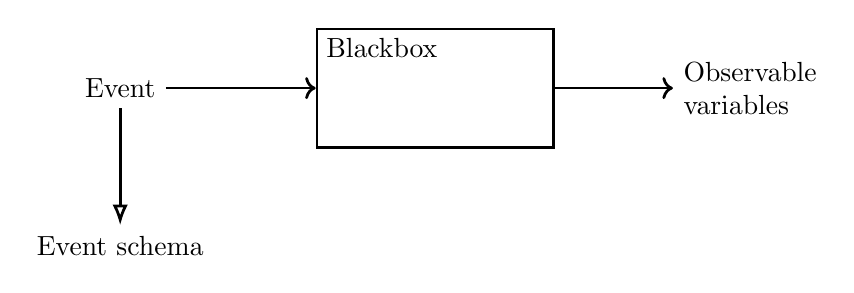
\begin{tikzpicture}[line width=1pt]
			\node [align=left] (Event) at (0,0) {Event};
			\node [draw,shape=rectangle,minimum width=3cm, minimum height=1.5cm] (Box) at (4,0)
				{};
			\node [anchor=north west] at (Box.north west) {Blackbox};
			\node [align=left] (Var) at (8, 0) {Observable\\ variables};
			\node [align=left] (Schema) at (0, -2) {Event schema};
			\draw[->] (Event) -- (Box);
			\draw[->] (Box) -- (Var);
			\draw[-{Latex[open]}] (Event) -- (Schema);
		\end{tikzpicture}

		\note<1->{Event schema: params + possible behaviours}
	
		\pause
		Test by Scenario: initial state and configuration + sequence of events

	\end{frame}

	\begin{frame}{Implementation}
		
		{\Large HOUSTON}

		\begin{itemize}
			\item<+-> Simplest possible implementation
			\item<+-> Input is subset of the possible CGS commands
			\item<+-> Verify by precondition-postcondition
			\item<+-> Timeout function required
		\end{itemize}

		\note{
		No preprogrammed missions, RC input, unintended events

		Precondition: circumstances

		Postcondition: consequences

		Expressed by observable variables
		}

	\end{frame}

	\begin{frame}{Preliminary results}
		Error:
		\begin{itemize}
			\item[] Arming copter twice makes future arm commands fail
		\end{itemize}

		\pause
		Test scenario:
		\begin{itemize}
			\item[] ARM $\rightarrow$ ARM $\rightarrow$ DISARM $\rightarrow$ ARM
		\end{itemize}
		\note{last postcondition would fail as copter would remain unarmed}
	\end{frame}

	\begin{frame}{Preliminary results}
		Error:
		\begin{itemize}
			\item[] Parachute command results in unwanted motor test
		\end{itemize}

		\pause
		Test scenario:
		\begin{itemize}
			\item[] Static configuration: enable parachute feature
			\item[] DISARM $\rightarrow$ PARACHUTE
		\end{itemize}
		\note{last postcondition would fail as copter would be armed}
	\end{frame}

%---------------------------------
% Section Threads to Validity
%---------------------------------
\section{Threads to Validity}
	\begin{frame}{Threads to Validity}
		TtV
	\end{frame}

%---------------------------------
% Section Conclusion \& Future work
%---------------------------------
\section{Conclusion \& Future work}
	\begin{frame}{Conclusion \& Future work}
		Conclusion
	\end{frame}

\begin{frame}[standout]

	{\Large Any questions?}

\end{frame}

% \fontsize{6pt}{7.2}\selectfont
\bibliographystyle{./aux/IEEEtranN}
\bibliography{./aux/IEEEabrv,lit}

\end{document}
